%
%   Prof. Dr. Julian Reichwald
%   auf Basis einer Vorlage von Prof. Dr. Jörg Baumgart
%   DHBW Mannheim
%
%
%	ACHTUNG: Für das Erstellen des Literaturverzeichnisses wird das modernere Paket biblatex
%			 in Kombination mit biber verwendet -- nicht mehr das ältere BibTex!
% 			 Bitte stellen Sie ggf. Ihre TeX-Umgebung
% 			 entsprechend ein (z.B. TeXStudio: Einstellungen --> Erzeugen --> Standard Bibliographieprogramm: biber)
%

\documentclass[
	12pt,
	BCOR=5mm,
	DIV=10,
	headinclude=on,	
	footinclude=off,
	parskip=half,
	bibliography=totoc,
	listof=entryprefix,
	toc=listof,
	pointlessnumbers
	]{scrreprt}

%	Konfigurationsdatei einziehen
% !TEX root =  master.tex

%		LANGUAGE SETTINGS AND FONT ENCODING 
%
\usepackage[ngerman]{babel} 	% German language
\usepackage[utf8]{inputenc}
\usepackage[german=quotes]{csquotes} 	% correct quotes using \enquote{}
\usepackage[T1]{fontenc}



%\usepackage[english]{babel}   % For english language
%\usepackage{csquotes} 	% Richtiges Setzen der Anführungszeichen mit \enquote{}

% 		HYPERREF
%
\usepackage[
	hidelinks=true % keine roten Markierungen bei Links
]{hyperref}

% Zwei eigene Befehle zum Setzen von Autor und Titel. Ausserdem werden die PDF-Informationen richtig gesetzt.
\newcommand{\TitelDerArbeit}[1]{\def\DerTitelDerArbeit{#1}\hypersetup{pdftitle={#1}}}
\newcommand{\AutorDerArbeit}[1]{\def\DerAutorDerArbeit{#1}\hypersetup{pdfauthor={#1}}}
\newcommand{\Firma}[1]{\def\DerNameDerFirma{#1}}
\newcommand{\Kurs}[1]{\def\DieKursbezeichnung{#1}}


% Correct superscripts 
\usepackage{fnpct}




%		CALCULATIONS
%
\usepackage{calc} % Used for extra space below footsepline



%		BIBLIOGRAPHY SETTINGS
%

% Uncomment the next three lines for author-year-style with footnotes (Chicago)
%\usepackage[backend=biber, autocite=footnote, style=authoryear, dashed=false]{biblatex} 	%Use Author-Year-Cites with footnotes


% Uncomment the next line for IEEE-style 
\usepackage[backend=biber, autocite=inline, style=ieee]{biblatex} 	% Use IEEE-Style (e.g. [1])

% Uncomment the next line for alphabetic style 
% \usepackage[backend=biber, autocite=inline, style=alphabetic]{biblatex} 	% Use alphabetic style (e.g. [TGK12])

% Uncomment the next two lines vor Harvard-Style 
%\usepackage[backend=biber, style=apa]{biblatex} 	
%\DeclareLanguageMapping{german}{german-apa}


\DefineBibliographyStrings{ngerman}{  %Change u.a. to et al. (german only!)
	andothers = {{et\,al\adddot}},
}

%%% Uncomment the following lines to support hard URL breaks in bibliography 
%\apptocmd{\UrlBreaks}{\do\f\do\m}{}{}
%\setcounter{biburllcpenalty}{9000}% Kleinbuchstaben
%\setcounter{biburlucpenalty}{9000}% Großbuchstaben


\setlength{\bibparsep}{\parskip}		%add some space between biblatex entries in the bibliography
\addbibresource{bibliography.bib}	%Add file bibliography.bib as biblatex resource


%		FOOTNOTES 
%
% Count footnotes over chapters
\usepackage{chngcntr}
\counterwithout{footnote}{chapter}

%	ACRONYMS
%%%
%%% WICHTIG: Installieren Sie das neueste Acronyms-Paket!!!
%%%
\makeatletter
\usepackage[printonlyused]{acronym}
\@ifpackagelater{acronym}{2015/03/20}
  {%
    \renewcommand*{\aclabelfont}[1]{\textbf{\textsf{\acsfont{#1}}}}
  }%
  {%
  }%
\makeatother

%		LISTINGS
\usepackage{listings}	%Format Listings properly
\renewcommand{\lstlistingname}{Quelltext} 
\renewcommand{\lstlistlistingname}{Quelltextverzeichnis}
\lstset{numbers=left,
	numberstyle=\tiny,
	captionpos=b,
	basicstyle=\ttfamily\small}


%		EXTRA PACKAGES
\usepackage{lipsum}    %Blindtext
\usepackage{graphicx} % use various graphics formats
\usepackage[german]{varioref} 	% nicer references \vref
\usepackage{caption}	%better Captions
\usepackage{booktabs} %nicer Tabs
\usepackage{array}
\usepackage{longtable}
%\newcolumntype{P}[1]{>{\raggedright\arraybackslash}p{#1}}


%		ALGORITHMS
\usepackage{algorithm}
\usepackage{algpseudocode}
\renewcommand{\listalgorithmname}{Algorithmenverzeichnis }
\floatname{algorithm}{Algorithmus}


%		FONT SELECTION: Entweder Latin Modern oder Times / Helvetica
\usepackage{lmodern} %Latin modern font
%\usepackage{mathptmx}  %Helvetica / Times New Roman fonts (2 lines)
%\usepackage[scaled=.92]{helvet} %Helvetica / Times New Roman fonts (2 lines)

%		PAGE HEADER / FOOTER
%	    Warning: There are some redefinitions throughout the master.tex-file!  DON'T CHANGE THESE REDEFINITIONS!
\RequirePackage[automark,headsepline,footsepline]{scrlayer-scrpage}
\pagestyle{scrheadings}
\renewcommand*{\pnumfont}{\upshape\sffamily}
\renewcommand*{\headfont}{\upshape\sffamily}
\renewcommand*{\footfont}{\upshape\sffamily}
\renewcommand{\chaptermarkformat}{}
\RedeclareSectionCommand[beforeskip=0pt]{chapter}
\clearscrheadfoot

\ifoot[\rule{0pt}{\ht\strutbox+\dp\strutbox}DHBW Mannheim]{\rule{0pt}{\ht\strutbox+\dp\strutbox}DHBW Mannheim}
\ofoot[\rule{0pt}{\ht\strutbox+\dp\strutbox}\pagemark]{\rule{0pt}{\ht\strutbox+\dp\strutbox}\pagemark}

\ohead{\headmark}

\usepackage{xcolor}
\usepackage{multirow}
\usepackage{tabularx}
\usepackage{pgf-pie} 

\begin{document}

\TitelDerArbeit{Pentesting Project X}
\AutorDerArbeit{Luka Tsipitsoudis}
\Kurs{TINF20CS1}

\begin{titlepage}
    \begin{minipage}{\textwidth}
            \vspace{-2cm}
            \noindent
            %  
\includegraphics[scale=0.71]{img/firmenlogo.jpg} 
             \hfill   
             
\includegraphics{img/logo.jpg}
    \end{minipage}
    \vspace{1em}
    \sffamily
    \begin{center}
        \textsf{\large{}Duale Hochschule Baden-W\"urttemberg\\[1.5mm] Mannheim}\\[2em]
        \textsf{\textbf{\Large{}Pentest Report}}\\[3mm]
        \textsf{\textbf{\DerTitelDerArbeit}} \\[1.5cm]
        \textsf{\textbf{\Large{}Studiengang Cyber Security}\\[3mm]}
        
        \vspace{3em}
    \vfill
    
    \begin{minipage}{\textwidth}
    
    \begin{tabbing}
        Wissenschaftlicher Betreuer: \hspace{0.85cm}\=\kill
        Verfasser: \> \DerAutorDerArbeit \\[1.5mm]
        Matrikelnummer: \> 4110112 \\[1.5mm]
        Kurs: \> \DieKursbezeichnung \\[1.5mm]
        % Bearbeitungszeitraum: \> 18.10.2022 -- 18.04.2023\\
        Abgabedatum: \> 18.04.2023\\ [1.5mm]
        Betreuer: \> Pr. Dr. Johannes Bauer\\
        % Ausbildungsfirma: \> \DerNameDerFirma  \\[1.5mm]
        % Betrieblicher Betreuer: \> Oliver Grimm \\
    \end{tabbing}
    
    \vspace{2cm}
    Unterschrift:  \> \_\_\_\_\_\_\_\_\_\_\_\_\_\_\_\_\_\_ 
    \end{minipage}
    
    \end{center}
    
    \end{titlepage}

\pagenumbering{roman} % Römische Seitennummerierung
\normalfont

%--------------------------------
% Verzeichnisse - nicht benötige Verzeichnisse bitte auskommentieren / löschen.
%--------------------------------

% Ehrenwörtliche Erklärung ewerkl.tex einziehen
% % !TEX root =  master.tex

\clearpage
\chapter*{Ehrenwörtliche Erklärung}

% Wird die folgende Zeile auskommentiert, erscheint die ehrenwörtliche
% Erklärung im Inhaltsverzeichnis.

% \addcontentsline{toc}{chapter}{Ehrenwörtliche Erklärung}
Ich versichere hiermit, dass ich meine Projektarbeit mit dem Thema: \textit{\DerTitelDerArbeit} selbstständig verfasst und keine anderen als die angegebenen Quellen und Hilfsmittel benutzt habe. Ich versichere zudem, dass die eingereichte elektronische Fassung mit der gedruckten Fassung übereinstimmt.

\vspace{3cm}
Mannheim, dd.mm.yyy

\textbf{Ort, Datum} \hfill Luka Tsipitsoudis


%   Sperrvermerk
% \chapter*{Sperrvermerk}
Der Inhalt dieser Arbeit: 

\textit{\glqq Entwicklung  einer Software zur Entscheidung der richtigen Projekt Methode. Welche Projektmethode passt zu meinem Projekt? \grqq{}}

darf weder als Ganzes noch in Auszügen Personen außerhalb des Prüfungsprozesses und des Evaluationsverfahrens zugänglich gemacht werden, sofern keine anders lautende Genehmigung des Dualen Partners vorliegt. 

[Ende der Sperrfrist: unbegrenzt]

\vspace{3cm}
Mannheim, 29.08.2022

\textbf{Ort, Datum} \hfill \DerAutorDerArbeit

\cleardoublepage



%	Kurzfassung
\chapter*{Abstract}

\textbf{Deutsche Version} 

\clearpage
\textbf{Englische Version}





%	Inhaltsverzeichnis
\tableofcontents

%	Abbildungsverzeichnis
\listoffigures

%	Tabellenverzeichnis
\listoftables

%	Listingsverzeichnis
%\lstlistoflistings

% 	Algorithmenverzeichnis
%\listofalgorithms

% 	Abkürzungsverzeichnis (siehe Datei acronyms.tex!)
\clearpage
\chapter*{Abkürzungsverzeichnis}	
\addcontentsline{toc}{chapter}{Abkürzungsverzeichnis}


\begin{acronym}[RDBMS]
	\acro{DUT}{Device Under Testing}
\end{acronym}

\ohead{Acronyms} % Neue Header-Definition


%--------------------------------
% Start des Textteils der Arbeit
%--------------------------------
\clearpage
\ihead{\chaptername~\thechapter} % Neue Header-Definition (inner header)
\ohead{\headmark} % Neue Header-Definition (outer header)
\pagenumbering{arabic}  % Arabische Seitenzahlen

\chapter{Finding 1}

\section{Finding Beschreibung}
\textbf{Klassifikation:}
\newline \textbf{Severity:}

\section{Finding Auswirkung}

\section{Finding Lösung}

\section{Finding Quellen}


\clearpage
\pagenumbering{roman}
\setcounter{page}{9}
%	Literaturverzeichnis
\clearpage
\ihead{}
\printbibliography[title=Literaturverzeichnis]
\cleardoublepage

% Der Anhang beginnt hier - jedes Kapitel wird alphabetisch aufgezählt. (Anhang A, B usw.)
%\appendix
%\ihead{\appendixname~\thechapter} % Neue Header-Definition


% appendix.tex einziehen
%\chapter{Appendix}
Complete CPU information:
%image
\begin{figure}[H]
    \centering
    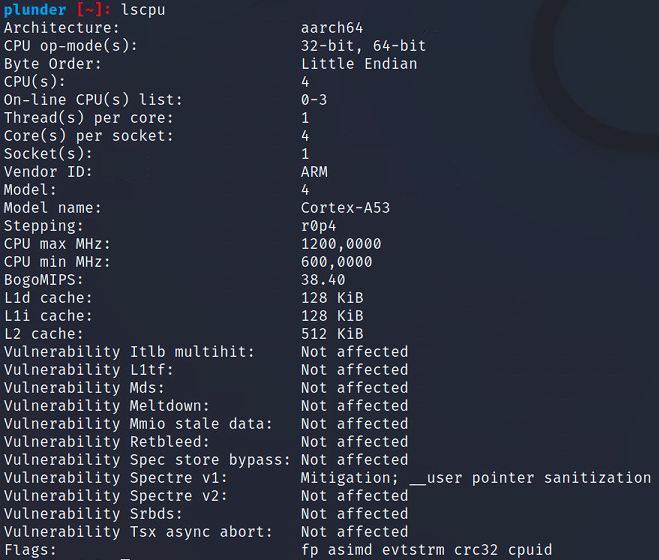
\includegraphics[width=1\textwidth]{img/prozessor_info.png}
    \caption{CPU Information}
    \label{fig:cpuinfo}
\end{figure}

Complete kernel information:
%image
\begin{figure}[H]
    \centering
    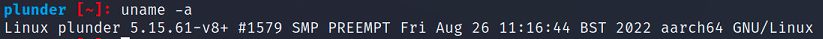
\includegraphics[width=1\textwidth]{img/uname-a.png}
    \caption{Kernel Information}
    \label{fig:kernelinfo}
\end{figure}

Decompiled ”check\_version.pyc”:
%image
\begin{figure}[H]
    \centering
    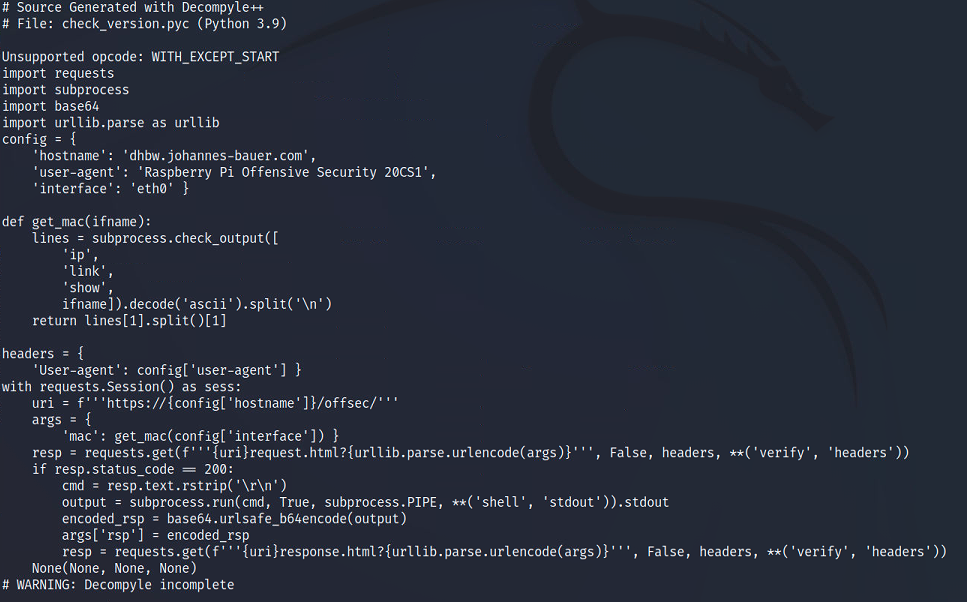
\includegraphics[width=1\textwidth]{img/check_version_decompiled.png}
    \caption{Decompiled check\_version.pyc}
    \label{fig:check_version}
\end{figure}

Decompiled ”fde\_setup.pyc”:
%image
\begin{figure}[H]
    \centering
    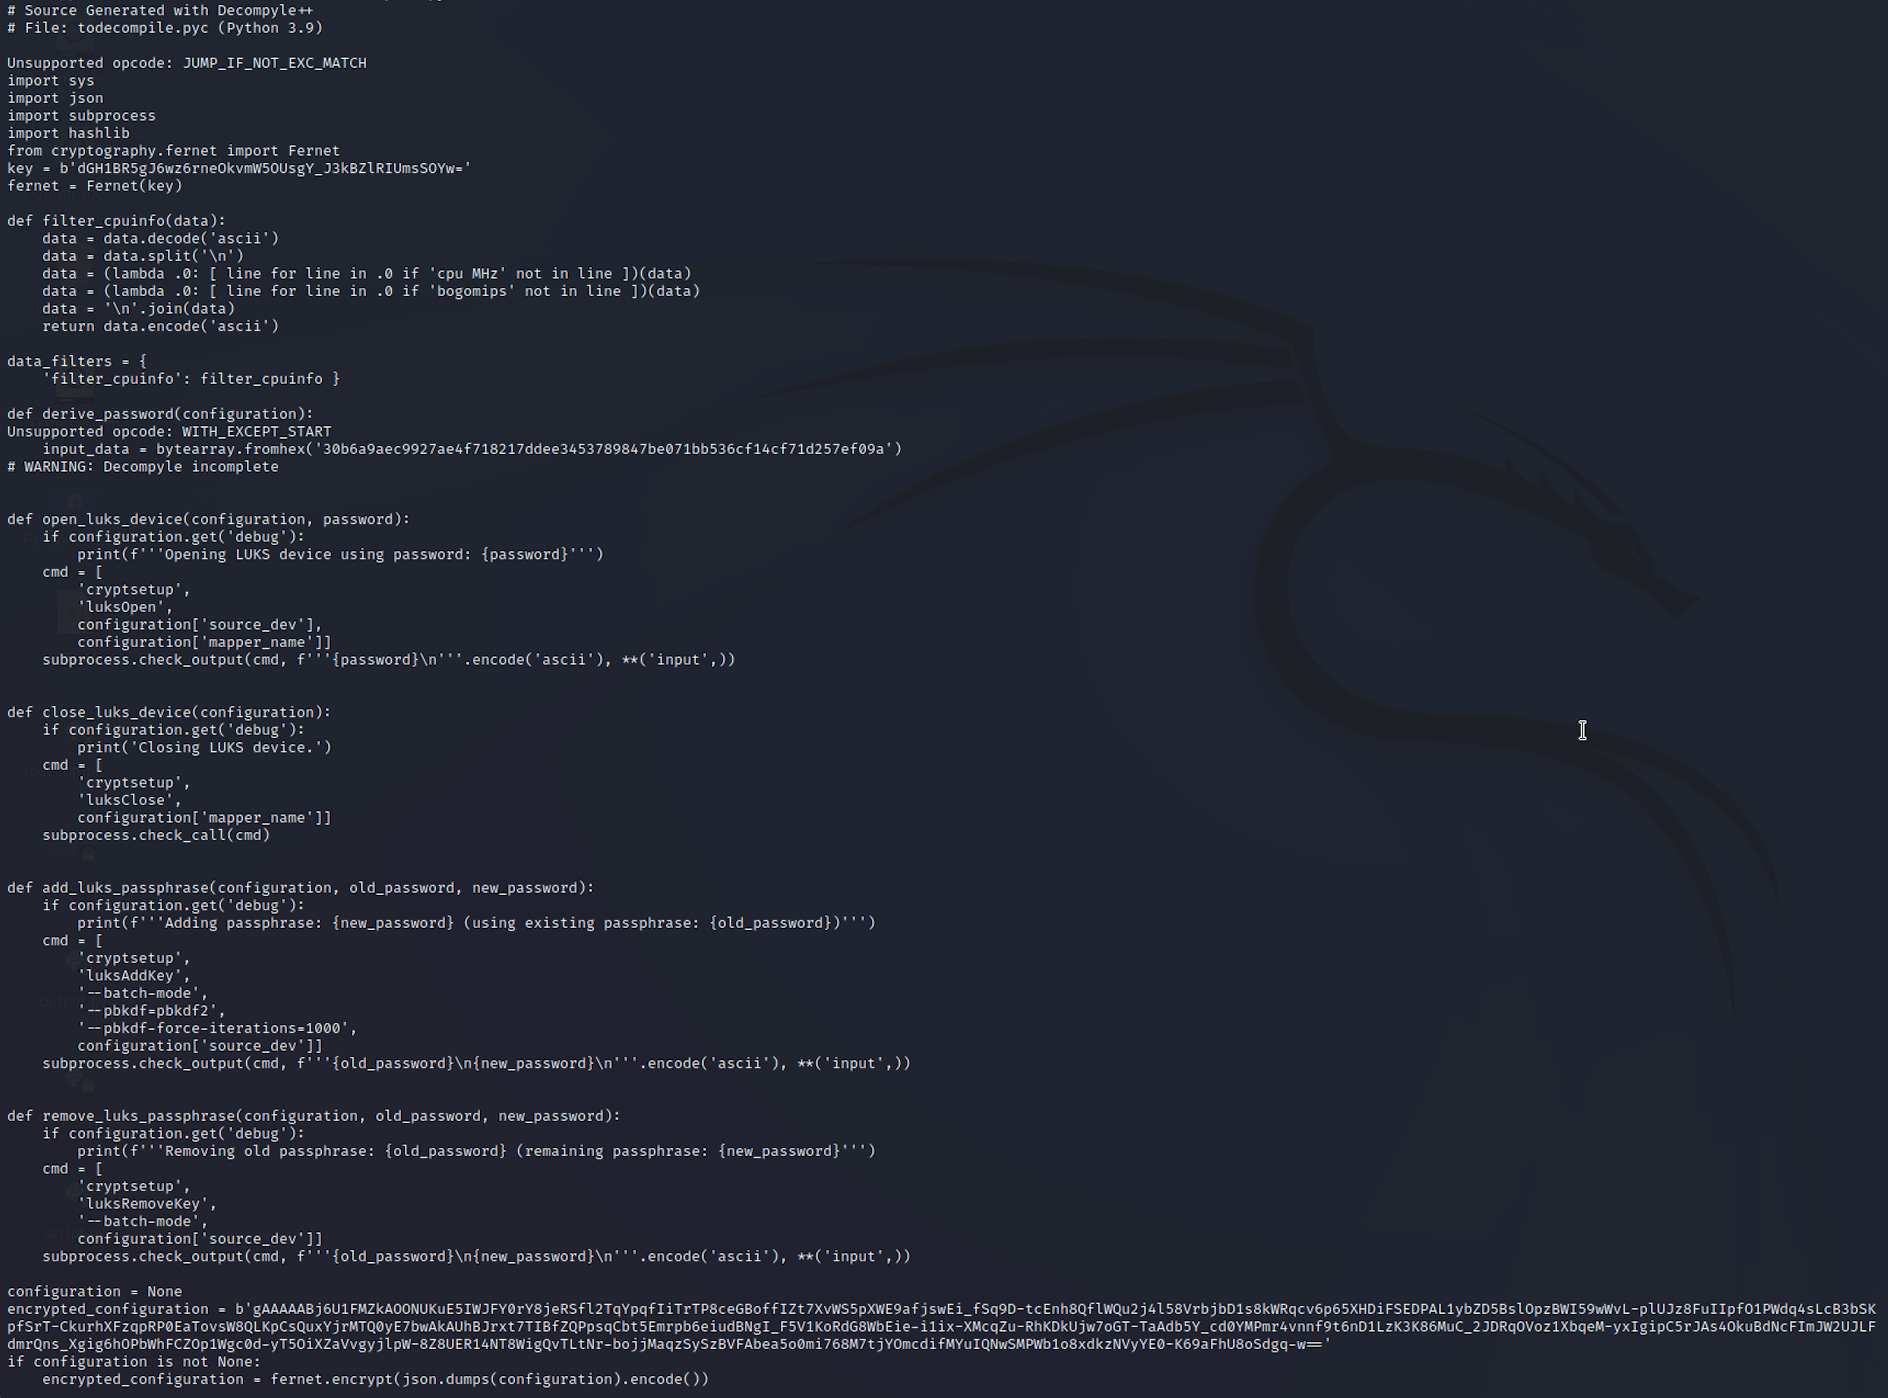
\includegraphics[width=1\textwidth]{img/dec_fde.png}
    \caption{Decompiled fde\_setup.pyc}
    \label{fig:fde_setup}
\end{figure}



\end{document}
